\documentclass[crop,tikz]{standalone}
\usepackage{siunitx}
\begin{document}
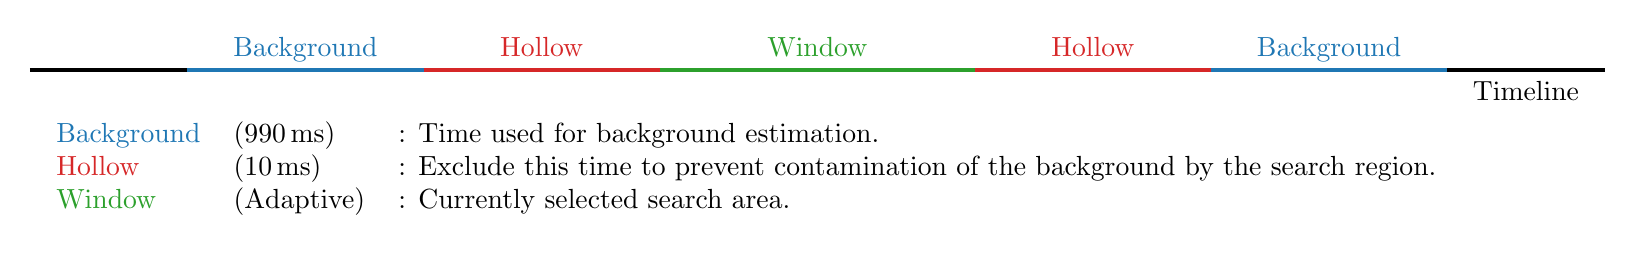
\begin{tikzpicture}
    \definecolor{C0}{HTML}{1f77b4}
    \definecolor{C2}{HTML}{2ca02c}
    \definecolor{C3}{HTML}{d62728}

    \coordinate (window_left) at (-2,0);
    \coordinate (window_right) at (2,0);
    \coordinate (exclude_left) at (-5,0);
    \coordinate (exclude_right) at (5,0);
    \coordinate (background_left) at (-8,0);
    \coordinate (background_right) at (8,0);
    \coordinate (timeline_left) at (-10,0);
    \coordinate (timeline_right) at (10,0);

    \coordinate (window_left_above) at (-2,1);
    \coordinate (window_right_above) at (2,1);

    \path[draw=black, ultra thick] (timeline_left) -- (background_left);
    \path[draw=black, ultra thick] (timeline_right) -- node[below] {Timeline} (background_right);
    \path[draw=C0, ultra thick] (background_left) -- node[above, anchor=base, yshift=5pt] {\textcolor{C0}{Background}} (exclude_left);
    \path[draw=C0, ultra thick] (exclude_right) -- node[above, anchor=base, yshift=5pt] {\textcolor{C0}{Background}} (background_right);
    \path[draw=C3, ultra thick] (exclude_left) -- node[above, anchor=base, yshift=5pt] {\textcolor{C3}{Hollow}} (window_left);
    \path[draw=C3, ultra thick] (window_right) -- node[above, anchor=base, yshift=5pt] {\textcolor{C3}{Hollow}} (exclude_right);
    \path[draw=C2, ultra thick] (window_left) -- node[above, anchor=base, yshift=5pt] {\textcolor{C2}{Window}} (window_right);

    \node at (-10,-0.5) [align=left, anchor=north west] {
        \begin{tabular}{lll}
            \textcolor{C0}{Background} & (\SI{990}{\milli\second}) & : Time used for background estimation.                                               \\
            \textcolor{C3}{Hollow}     & (\SI{10}{\milli\second})  & : Exclude this time to prevent contamination of the background by the search region. \\
            \textcolor{C2}{Window}     & (Adaptive)                & : Currently selected search area.
        \end{tabular}
    };

\end{tikzpicture}
\end{document}
